\documentclass[12pt,a4paper]{article}
\usepackage[UTF8]{ctex}     %先引入ctex
\usepackage[utf8]{inputenc} %再引入inputenc
\usepackage{graphicx}
% \usepackage{lazylatex}
% \tcbuselibrary{documentation}
\usepackage{amsmath}
\usepackage{bookmark}
\usepackage{enumerate}
\usepackage{geometry}
\graphicspath{{img/}}
% 边距
\geometry{left=2.0cm,right=2.0cm,top=2.0cm,bottom=3.0cm}
% 大题
\newenvironment{problems}{\begin{list}{}{\renewcommand{\makelabel}[1]{\textbf{##1}.\hfil}}}{\end{list}}
% 小题
\newenvironment{steps}{\begin{list}{}{\renewcommand{\makelabel}[1]{(##1)\hfil}}}{\end{list}}
% 答
\providecommand{\ans}{\textbf{答}:~}
% 解
\providecommand{\sol}{\textbf{解}.~}

% \setminted{breaklines,autogobble,frame=lines,framesep=2mm,fontsize=\scriptsize}

\begin{document}
\title{\normalsize \underline{计算机系统结构(A)}\\\LARGE 实验 4}
\author{李子龙 518070910095}
\date{\today}
\maketitle

\begin{problems}
    \item[一] \textbf{Cache 可视化工具}
    
    \begin{steps}
        \item[1] 场景一
        
        \begin{itemize}
            \item Cache 命中率为 0\% 。
            
            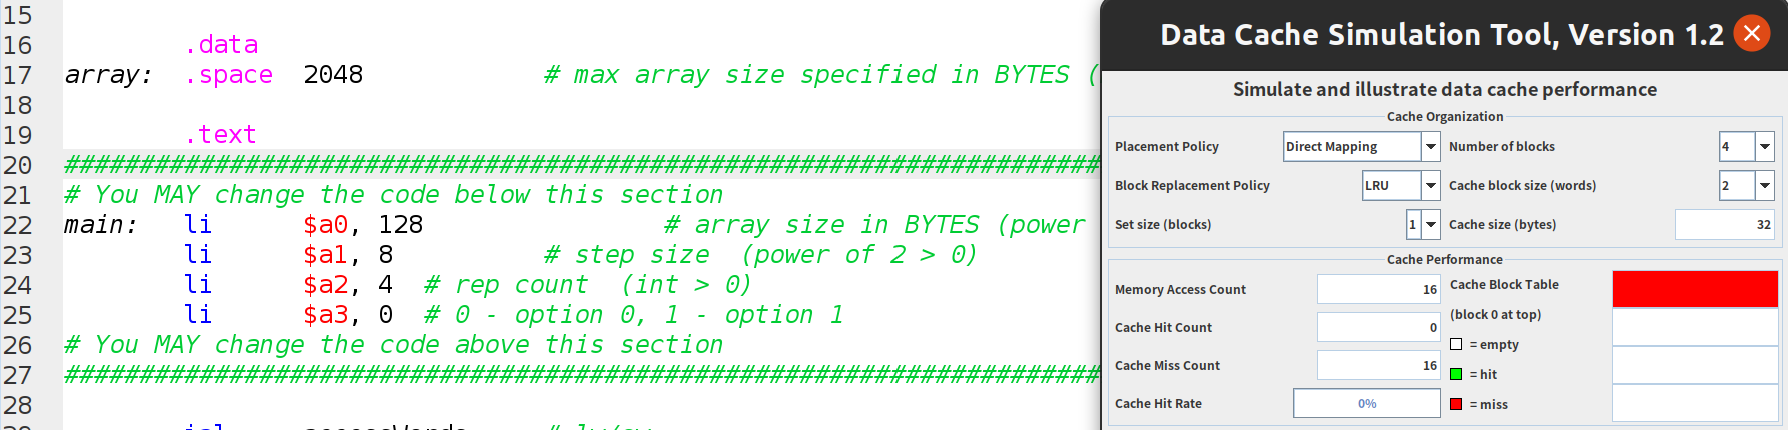
\includegraphics[width=0.7\textwidth]{cache1.png}
            \item \verb"stepsize" 被设定为 8,按照 \verb"int"(4 Bytes) 存储,写入(\verb"option"为0)需要跳跃 32 bytes,只有一组,而一组正好是
            \begin{equation*}
                4\text{ blocks}\times 2\text{ words}\times 4\text{ bytes} = 32 \text{ bytes}
            \end{equation*}
            将会导致每一次的写入都会失效。
            \item 增加 \verb"repcount" 也无法提高命中率,因为上文所述的间隔无法被改变,会一直失效。
            \item 将 \verb"stepsize" 更改为 1,可以将命中率提高至 50\% 。
            
            每对访问第一个失效,第二个命中,在块大小为 2 个字的情形下。

            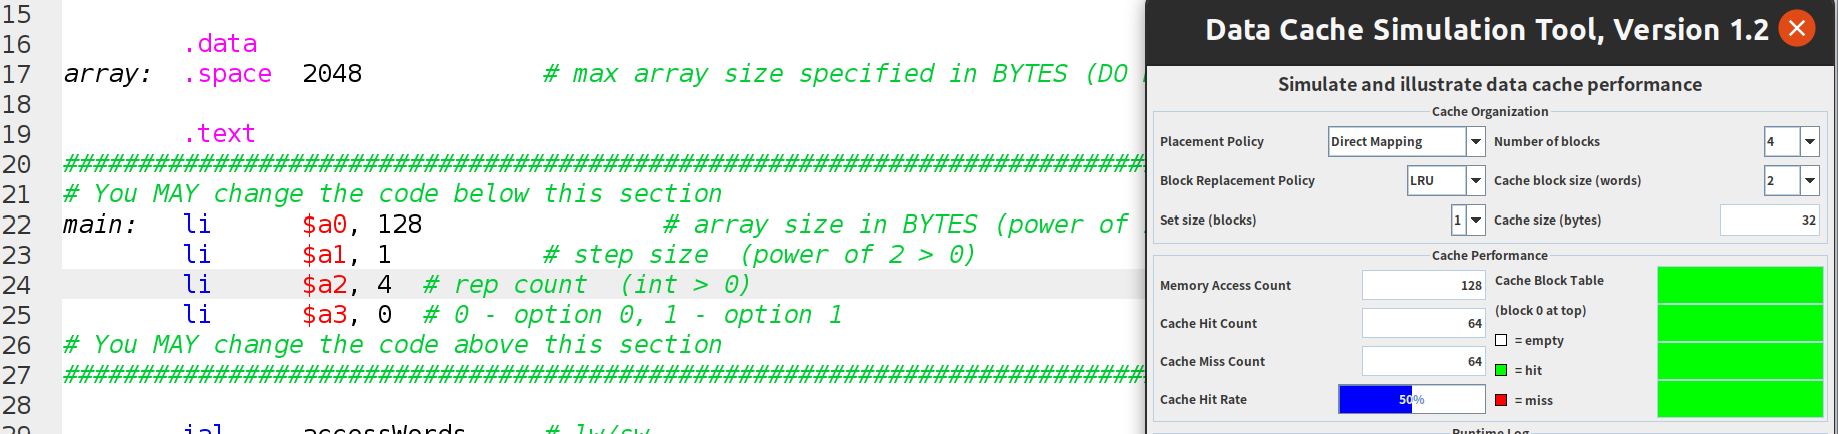
\includegraphics[width=0.7\textwidth]{cache1o.png}
        \end{itemize}

        \item[2] 场景二
        \begin{itemize}
            \item 命中率为 75 \% 。
            
            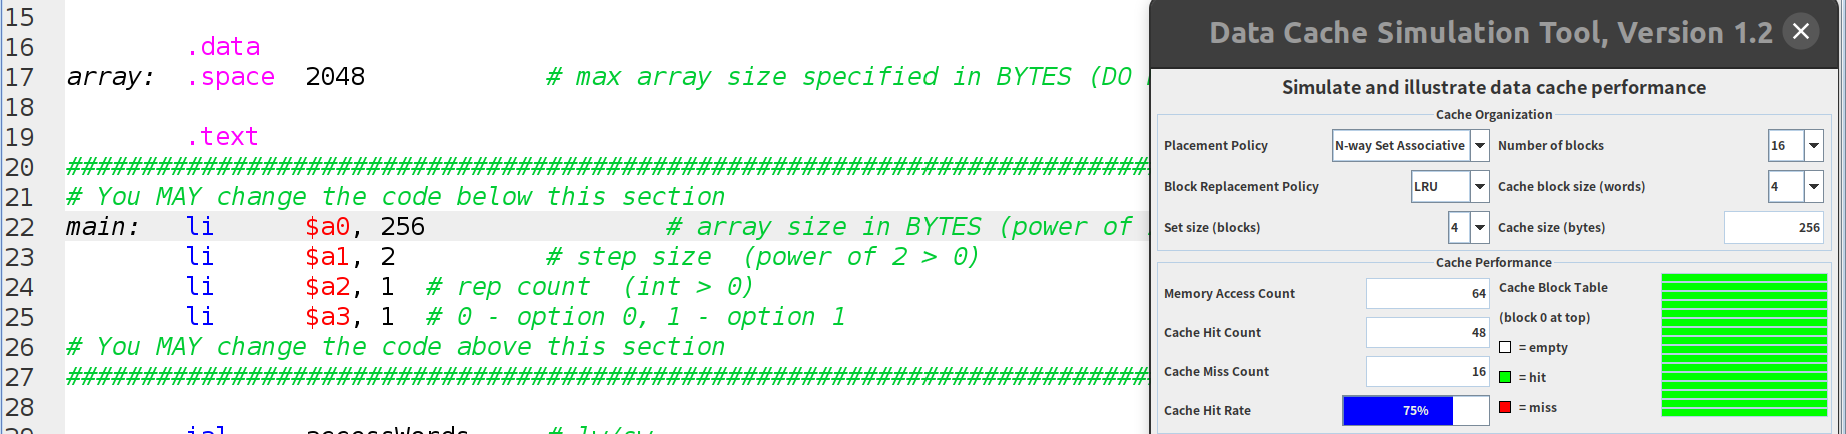
\includegraphics[width=0.7\textwidth]{cache2.png}
            \item \verb"stepsize" 是 2,一块 4 个字,那么相邻的两次读+写,除了第一个读失效,其余均为命中,命中率为 75\% 。
            \item 命中率会接近于 100\% 。因为以第一重复后,所有的数据都进入了 Cache,Cache 大小和数组大小相同:256 bytes,那么后面都不会失效。
            
            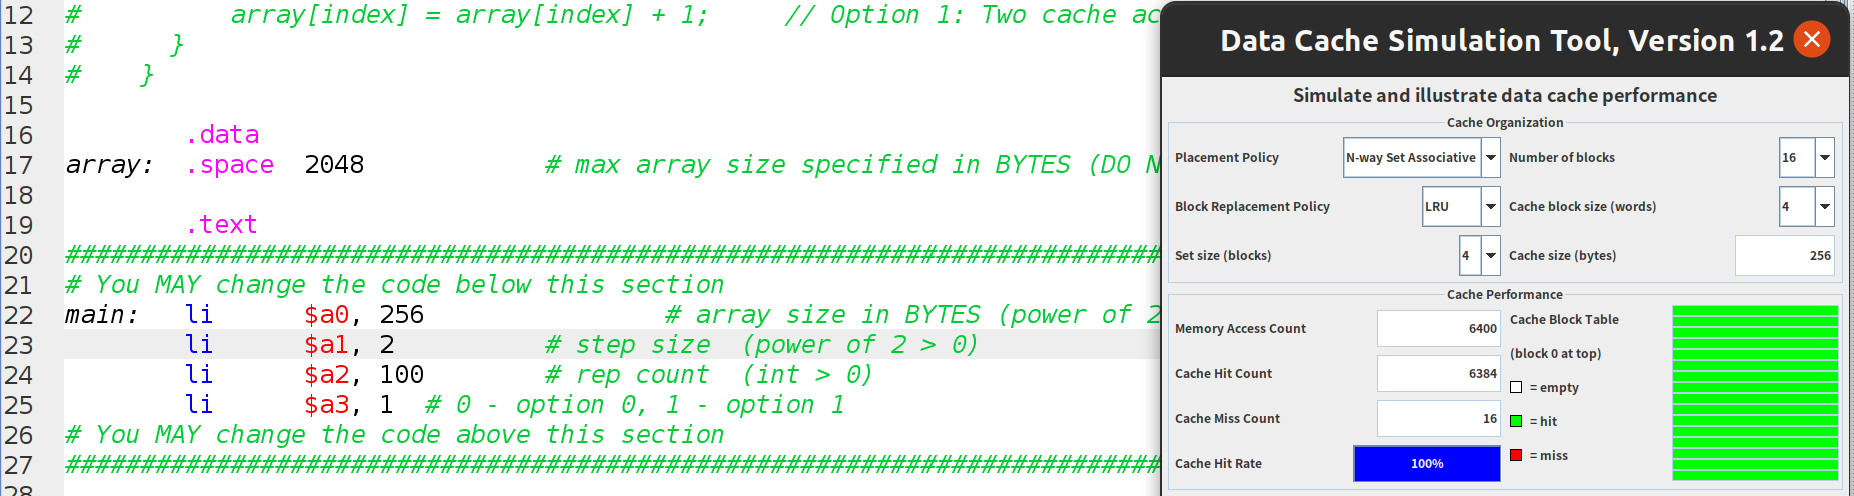
\includegraphics[width=0.7\textwidth]{cache2o.png}
        \end{itemize}
    \end{steps}
    
    \item[二] \textbf{矩阵乘法}
    \begin{itemize}
        \item ikj 性能最好,jki 性能最差。
        
        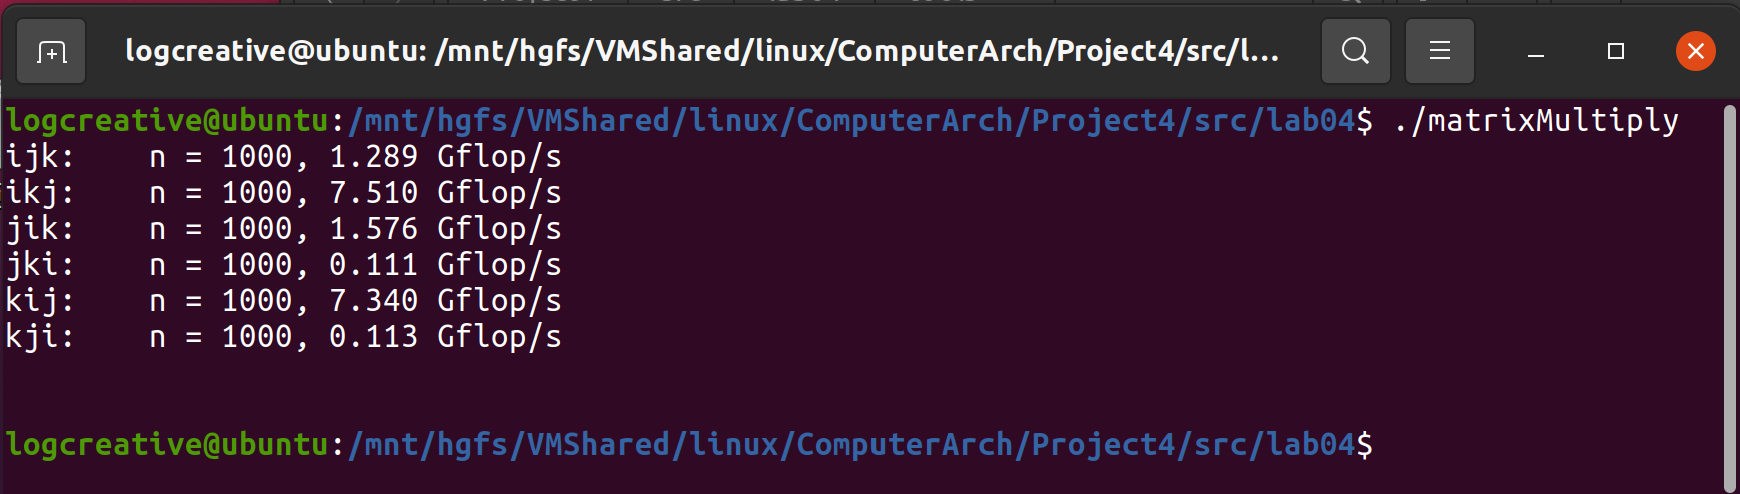
\includegraphics[width=0.8\textwidth]{matrix1.png}
    \end{itemize}
\end{problems}


\end{document}
